\documentclass[a4paper,12pt]{article} 
\usepackage[T2A]{fontenc}			
\usepackage[utf8]{inputenc}			
\usepackage[english,russian]{babel}	
\usepackage{amsmath,amsfonts,amssymb,amsthm,mathrsfs,mathtools} 
\usepackage{cancel}
\usepackage{multirow}
\usepackage[colorlinks, linkcolor = blue]{hyperref}
\usepackage{upgreek}\usepackage[left=2cm,right=2cm,top=2cm,bottom=3cm,bindingoffset=0cm]{geometry}
\usepackage{graphicx,wrapfig,subfig}
\usepackage{xcolor}
\author{Дорогинин Д.В.\\
Группа Б02-825}
\title{3.5.1. Изучение плазмы газового разряда в неоне.}
\date{}
\begin{document}
\maketitle
\textbf{Цель работы}: изучение вольт-амперной характеристики тлеющего разряда, изучение свойств плазмы методом зондовых характеристик.


\textbf{В работе используются}: стеклянная газоразрядная трубка, наполненная изотопом неона, высоковольтный источник питания (ВИП), источник питания постоянного тока, делитель напряжения, резистор, потенциометр, амперметры, вольтметры, переключатели.
\section*{Теория}
\subsection*{Плазма}
В ионизированном газе поле ионов <<экранируется>> электронами. Для поля $\mathbf{E}$ и плотности $\rho$ электрического заряда
$$
\text{div}~\mathbf{E} = 4 \pi \rho,
$$
а с учётом сферической симметрии и $\mathbf{E} = -\text{grad}~\varphi$:
\begin{equation}
\dfrac{d^2 \varphi}{dr^2}+\dfrac{2}{r}\dfrac{d\varphi}{dr}=-4\pi \rho.
\end{equation}
Плотности заряда электронов и ионов (которые мы считаем бесконечно тяжёлыми и поэтому неподвижными)
\begin{equation}
\begin{array}{c}
\rho_e = -ne \cdot \exp\left(\dfrac{e\varphi}{kT_e}\right),\\
\rho_i = ne.
\end{array}
\end{equation}
Тогда из $(1)$ в предположении $\dfrac{e\varphi}{kT_e} \ll 1$ получим
\begin{equation}
\varphi = \dfrac{Ze}{r}e^{-r/r_D},
\end{equation}
где $r_D = \sqrt{\dfrac{kT_e}{4\pi n e^2}}$ -- \textit{радиус Дебая}. Среднее число ионов в сфере такого радиуса 
\begin{wrapfigure}{r}{4cm}
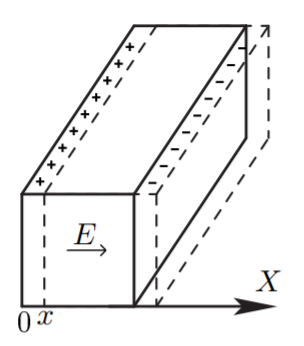
\includegraphics[scale=0.5]{2.png}
\end{wrapfigure}  
\begin{equation}
N_D = n\dfrac{4}{3}\pi r_D^2.
\end{equation}
Теперь выделим параллелепипед с плотностью $n$ электронов, сместим их на $x$. Возникнут поверхностные заряды $\sigma = nex$, поле от которых будет придавать электронам ускорение:
$$
\dfrac{d^2x}{dt^2}=-\dfrac{eE}{m}=-\dfrac{4\pi n e^2}{m}x.
$$ 
Отсюда получаем \textit{плазменную (ленгмюровскую) частоту} колебаний электронов:
\begin{equation}
\omega_p = \sqrt{\dfrac{4\pi ne^2}{m}}.
\end{equation}
\subsection*{Одиночный зонд}
При внесении в плазму уединённого проводника -- \textit{зонда} -- с потенциалом, изначально равным потенциалу точки плазмы, в которую его помещают, на него поступают токи электроннов и ионов:
\begin{equation}
\begin{array}{c}
I_{e0} = \dfrac{n \langle v_e \rangle}{4}eS,\\
I_{i0} = \dfrac{n \langle v_i \rangle}{4}eS,
\end{array}
\end{equation}
где $\langle v_e \rangle$ и $\langle v_i \rangle$ -- средние скорости электронов и ионов, $S$ -- площадь зонда, $n$ -- плотность электронов и ионов. Скорости электронов много больше скорости ионов, поэтому $I_{i0} \ll I_{e0}$. Зонд будет заряжаться до некоторого равновестного напряжения $-U_f$ -- \textit{плавающего потенциала}.\\
\begin{wrapfigure}{r}{5.5cm}
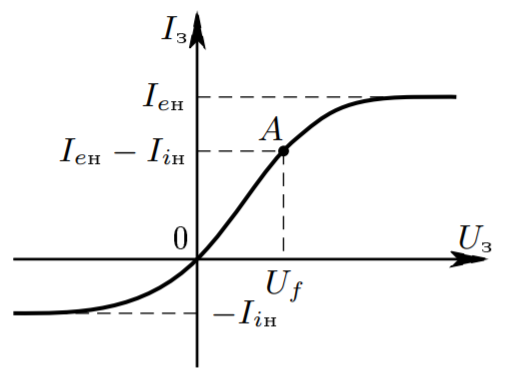
\includegraphics[scale=0.5]{3.png}
\end{wrapfigure}  
В равновесии ионный ток мало меняется, а электронный имеет вид
$$
I_e = I_0 \exp\left( -\dfrac{eU_f}{kT_e} \right).
$$
Будем подавать потенциал $U_\text{з}$ на зонд и снимать значение зондового тока $I_\text{з}$. Максимальное значение тока $I_{e\text{н}}$ -- электронный ток насыщения, а минимальное $I_{i\text{н}}$ -- ионный ток насыщения. Значение из эмпирической формулы Бомона:
\begin{equation}
I_{i\text{н}} = 0.4 neS \sqrt{\dfrac{2kT_e}{m_i}}.
\end{equation}
\subsection*{Двойной зонд}
Двойной зонд -- система из двух одинаковых зондов, расположенных на небольшом расстоянии друг от друга, между которыми создаётся разность потенциалов, меньшая $U_f$. Рассчитаем ток между ними вблизи $I=0$. При небольших разностях потенциалов ионные токи на оба зонда близки к току насыщения и компенсируют друг друга, а значит величина результирующего тока полностью связана с разностью электронных токов. Пусть потенциалы на зондах
$$
U_1 = -U_f + \Delta U_1,
$$
$$
U_2 = -U_f + \Delta U_2.
$$
Между зондами $U = U_2 - U_1 = \Delta U_2 - \Delta U_1$.
Через первый электрод
\begin{equation}
I_1 = I_{i\text{н}} + I_{e1} = I_{i\text{н}} - \dfrac{1}{4}neS\langle v_e\rangle \exp\left(-\dfrac{eU_f}{kT_e}\right)\exp\left(\dfrac{e\Delta U_1}{kT_e}\right)=I_{i\text{н}}\left(1 - \exp\left( \dfrac{e\Delta U_1}{kT_e} \right)\right).
\end{equation}
Аналогично через второй получим
\begin{equation}
I_2 = I_{i\text{н}}\left(1 - \exp\left( \dfrac{e\Delta U_2}{kT_e} \right)\right)
\end{equation}
  
Из $(7)$ и $(8)$ с учётом последовательного соединение зондов ($I_1 = -I_2 = I)$:
$$
\Delta U_1= \dfrac{kT_e}{e}\text{ln}\left(1 - \dfrac{I}{I_{i\text{н}}}\right)
$$
$$
\Delta U_2= \dfrac{kT_e}{e}\text{ln}\left(1 + \dfrac{I}{I_{i\text{н}}}\right)
$$

Тогда итоговые формулы для разности потенциалов и тока

\begin{equation}
U = \dfrac{kT_e}{e}\text{ln}\dfrac{1 - I/I_{i\text{н}}}{1 + I/I_{i\text{н}}}, 
I = I_{i\text{н}} \text{th}\dfrac{eU}{2kT_e}.
\end{equation}
Реальная зависимость выглядит несколько иначе и описывается формулой 
\begin{wrapfigure}{l}{7cm}
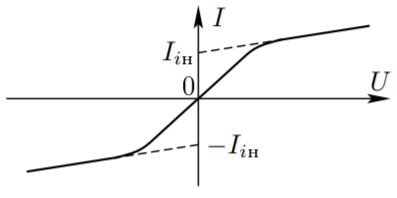
\includegraphics[scale=0.8]{4.png}
\vspace{+30pt}
\end{wrapfigure}
\begin{equation}
I = I_{i\text{н}} \text{th}\dfrac{eU}{2kT_e} + AU.
\end{equation}
Из этой формулы можно найти формулу для $T_e$: для $U=0$ мы найдём $I_{i\text{н}}$, продифференцируем в точке $U=0$ и с учётом $\text{th}~\alpha \approx \alpha$ при малых $\alpha$ и $A\rightarrow 0$ получим:
\begin{equation}
kT_e = \dfrac{1}{2}\dfrac{eI_{i\text{н}}}{\dfrac{dI}{dU}|_{U=0}}.
\end{equation}
\section*{Описание установки}
\begin{center}
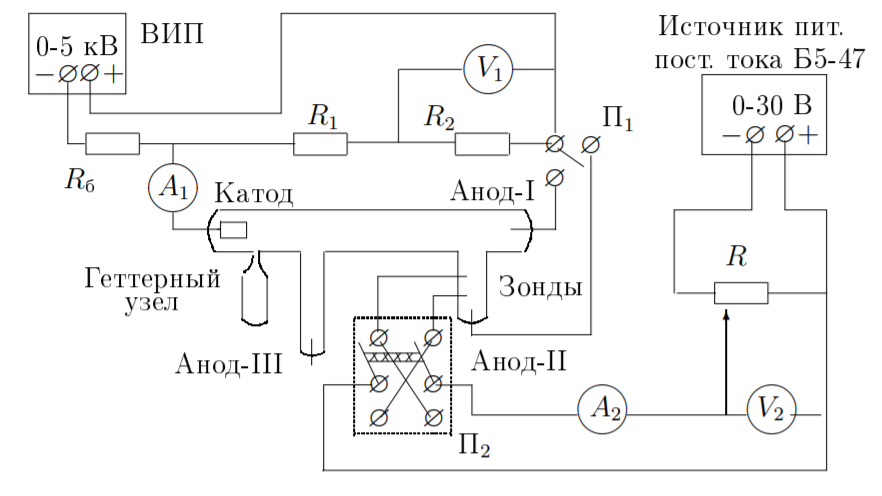
\includegraphics[scale=0.6]{1.png}
\end{center}
Стеклянная газоразрядная трубка имеет холодный (ненакаливаемый) полый катод, три анода и \textit{геттерный} узел -- стеклянный баллон, на внутреннюю повехность которого напылена газопоглощающая плёнка (\textit{геттер}). Трубка наполнена изотопом неона $^22$Ne при давлении 2 мм рт. ст. Катод и один из анодом (I и II) с помощью переключателя $\Pi_1$ подключается через балластный резистор $R_\text{б}$ ($\approx 450$ кОм) к регулируемому ВИП с выкодным напряжением до 5 кВ.\\
При подключении к ВИП анода-I между ним и катодом возникает газовый разряд. Ток разряда измеряется миллиамперметром $A_1$, а падение напряжения на разрядной трубке -- цифровым вольтметром $V_1$, подключённым к трубке черезе высокоомный (25 МОм) делитель напряжения с коэффициентом $(R_1+R_2)/R_2 = 10$.\\
При подключении к ВИП анода-II разряд возникает в пространстве между катодом и анодом-II, где находятся двойной зонд, используемый для диагностики плазмы положительного столба. Зонды изготовлены из молибденовой проволоки диаметром $d = 0.2$ мм и имеют длину $l = 5.2$ мм. Они подключены к источнику питания GPS через потенциометр $R$. Переключатель $\Pi_2$ позволяет изменять полярность напряжения на зондах. Величина напряжения на зондах изменяеься с помощью дискретного переключателя <<$V$>> выходного напряжения источника питания и потенциометра $R$, а измеряется цифровым вольтметром $V_2$. Для измерения зондового тока используется мультиметр $A_2$.
\section*{Ход работы}
Измеряем напряжение зажигания в лампе: $U_{\text{заж}} = 25.7\pm 0.2$ В.\\
С помощью вольтметра $V_1$ и амперметра $A_1$ снимаем ВАХ разряда $U_1=f(I_p)$ для тока в диапазоне $0.5 \div 5$ мА (см. Таблица 1).
Построим график:\\
\begin{figure}[h]
\centering
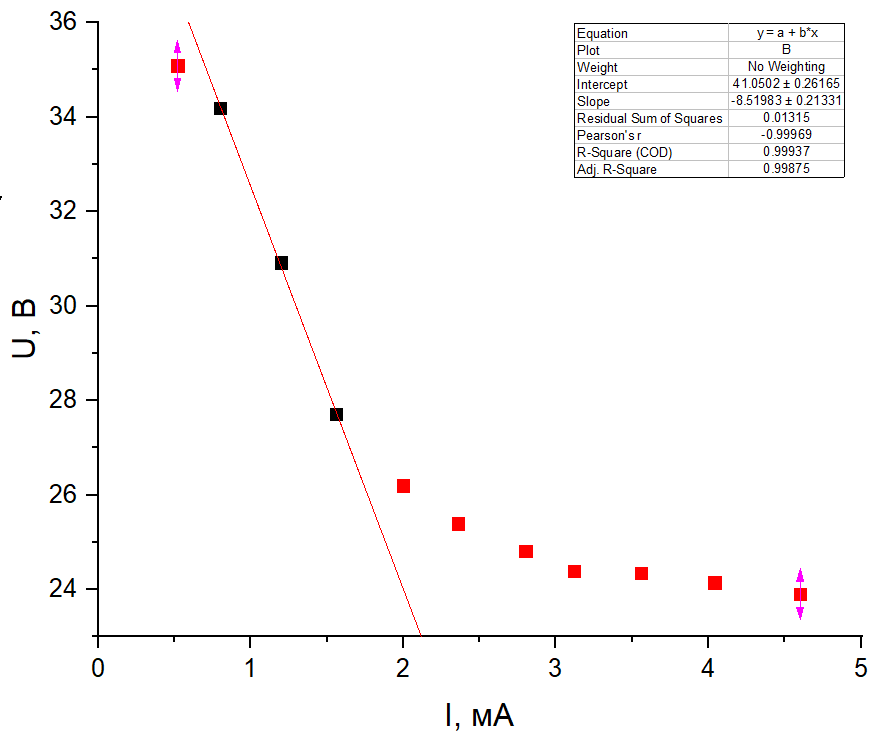
\includegraphics[scale=0.6]{6.png}
\caption{Вольт-амперная характеристика разряда.}
\end{figure}\\
По наклону определим максимальное сопротивление заряда (с учётом того, что вольтметр подключен через делитель напряжения с коэффициентом 10): $R_{max} = (8.5\pm 0.2)\cdot 10^4~\text{Ом}$.\\
С помощью вольтмертра $V_2$ и амперметра $A_2$ снимем ВАХ двойного зонда $I_2 = f(U_2)$ при фиксированного токе разряда $I_p$ в трубке в диапозоне $-25 \div 25$ В, процессе измерений меняя полярность зонда при нулевом токе. Измерения проведём для $I_p = 5$ мА, $I_p = 3$ мА  и $I_p = 1.5$ мА (Таблица 2).\\
Результаты измерений представим на графиках с отцентрованными $\left(I_0 = \dfrac{1}{2}\sum I\right)$:
\newpage
\begin{figure}[h]
    \centering
    \subfloat[ВАХ двойного зонда, $I = 5.0$ мА.]{{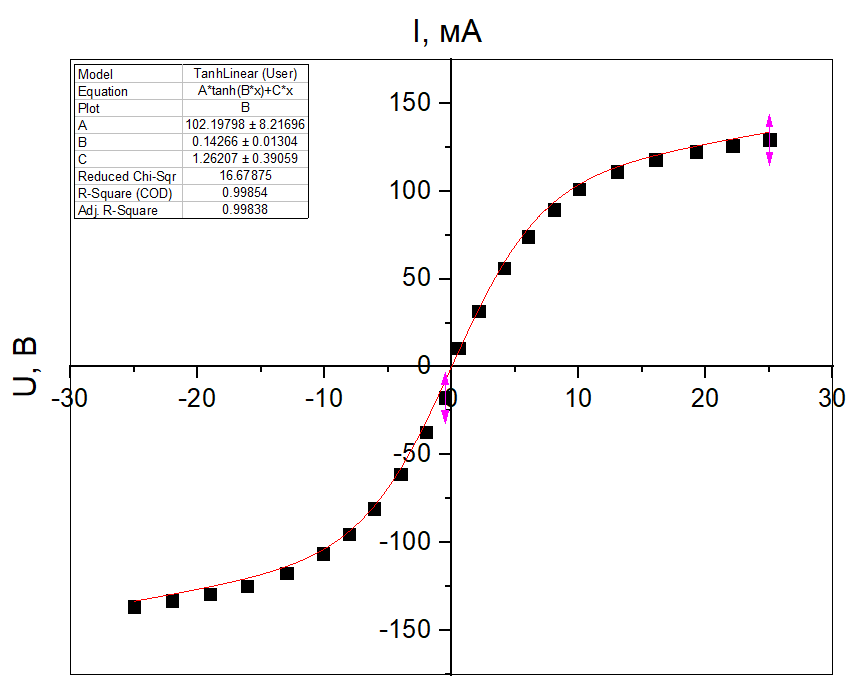
\includegraphics[width=0.5\textwidth]{5.png}}}
    \subfloat[ВАХ двойного зонда, $I = 3.0$ мА.]{{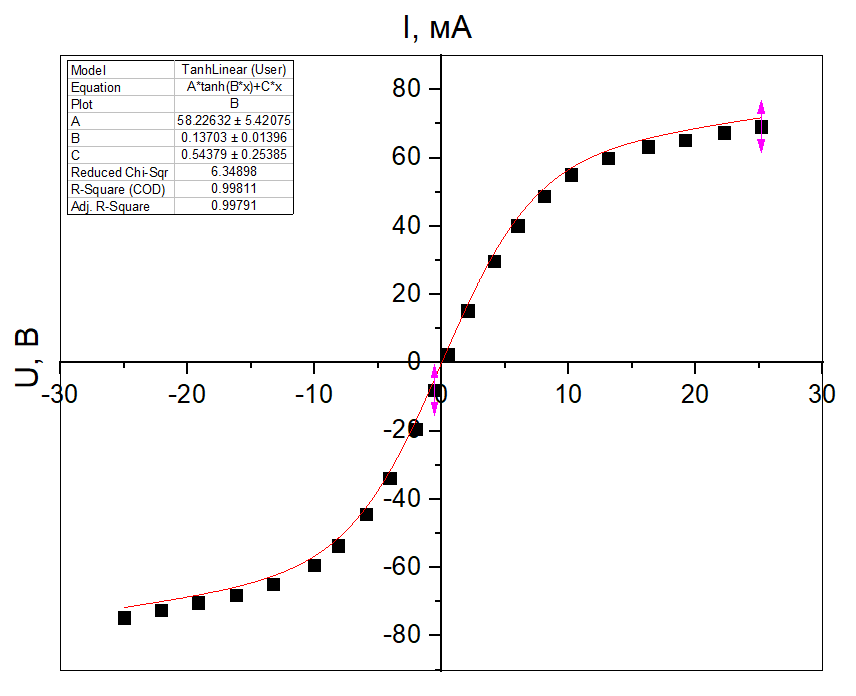
\includegraphics[width=0.5\textwidth]{7.png}}}\\
    \subfloat[ВАХ двойного зонда, $I = 1.5$ мА.]{{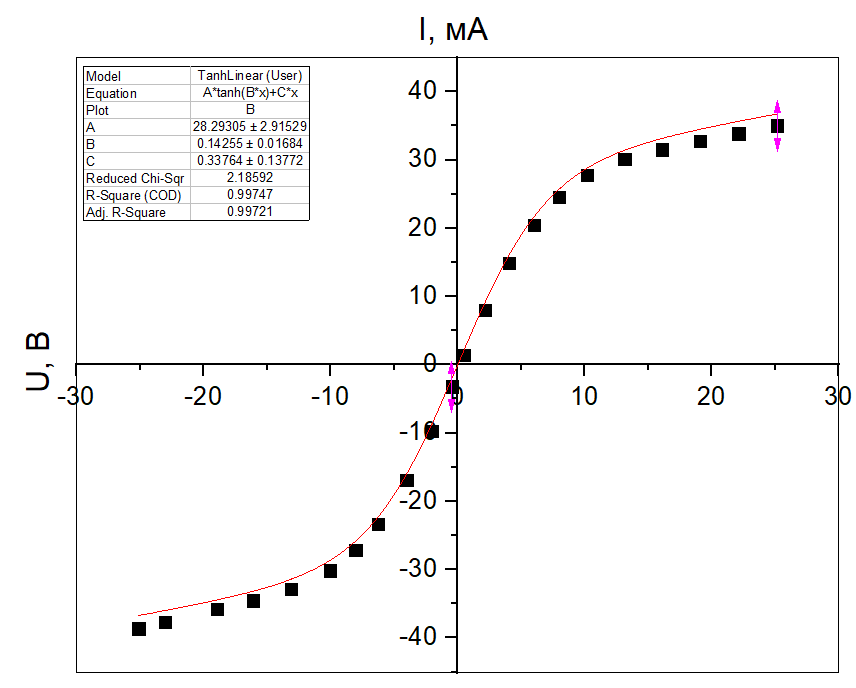
\includegraphics[width=0.5\textwidth]{8.png}}}
\end{figure}
Приближая кривые формулой $I = A \text{th}(BU) + CU$, найдём токи насыщения $I_{i\text{н}}$ и температуры электронов $T_e$.\\
Считая концентрации ионов и электронов равными, найдём их, пользуясь формулой (7). Рассчитаем плазменную частоты $\omega_p$ по формуле (5) и радиус Дебая $r_D$, оценим среднее число ионов в дебаевской сфера $N_D$ по формуле (4) и  степень ионизации $\alpha$, приняв $P\approx 1$ мбар, и занесём все результаты в таблицу.
\begin{table}[h!]
\centering
\begin{tabular}{|c|c|c|c|c|c|c|}
\hline
$I_p$, мА  & $T_e$, $10^4$ К   & $n_e$, $10^{15}$ м$^{-3}$ & $\omega_p$, $10^4$ рад/c & $r_D$, $10^{-5}$ см & $N_D$ & $\alpha$, $10^{-7}$ \\ \hline
5.0   & $41\pm 4$ & $58\pm 6$                     & $144\pm 10$                   & $49\pm 3$                      & 30 & 24\\ \hline
3.0   & $42\pm 4$ & $33\pm 4$                     & $107\pm 9$                    & $66\pm 5$                      & 40 & 13\\ \hline
1.5   & $41\pm 6$ & $16\pm 2$                    & $75\pm 8$                     & $94 \pm 10$                     & 57 & 7\\ \hline
\end{tabular}
\end{table}
\newpage
\section*{Результаты измерений}
\begin{table}[h]
\centering
\begin{tabular}{|c|c|c|c|c|c|c|c|c|c|c|c|}
\hline
$U_1$, В & 23.9 & 24.15 & 24.35 & 24.4 & 24.81 & 25.40 & 26.20 & 27.71 & 30.92 & 34.19 & 35.09 \\ \hline
$I_p$, мА & 4.60 & 4.04  & 3.56  & 3.12 & 2.80  & 2.36  & 2.00  & 1.56  & 1.20  & 0.80  & 0.52  \\ \hline
\end{tabular}
\caption{Зависимость $U_1 = f(I_p)$.}
\end{table}


\begin{table}[h]
\centering
\begin{tabular}{|c|c|c|c|c|c|c|c|}
\cline{1-2} \cline{4-5} \cline{7-8}
\multicolumn{2}{|c|}{$I_p = 5.0$ мА} &  & \multicolumn{2}{c|}{$I_p = 3.0$ мА} &  & \multicolumn{2}{c|}{$I_p = 1.5$ мА} \\ \cline{1-2} \cline{4-5} \cline{7-8} 
$U_2$, В          & $I_2$, мкА        &  & $U_2$, В         & $I_2$, мкА        &  & $U_2$, В          & $I_2$, мкА         \\ \cline{1-2} \cline{4-5} \cline{7-8} 
25.01          & 126.20          &  & 25.13         & 66.86          &  & 25.15          & 33.67           \\ \cline{1-2} \cline{4-5} \cline{7-8} 
22.11          & 122.84         &  & 22.23         & 65.03          &  & 22.09          & 32.50           \\ \cline{1-2} \cline{4-5} \cline{7-8} 
19.23          & 119.52         &  & 19.14         & 62.97          &  & 19.06          & 31.36           \\ \cline{1-2} \cline{4-5} \cline{7-8} 
16.04          & 114.79         &  & 16.23         & 60.95          &  & 16.09          & 30.18           \\ \cline{1-2} \cline{4-5} \cline{7-8} 
13.02          & 108.13         &  & 13.12         & 57.65          &  & 13.13          & 28.78           \\ \cline{1-2} \cline{4-5} \cline{7-8} 
10.00          & 97.96          &  & 10.21         & 52.78          &  & 10.18          & 26.37           \\ \cline{1-2} \cline{4-5} \cline{7-8} 
8.04           & 86.26          &  & 8.04          & 46.57          &  & 7.98           & 23.24           \\ \cline{1-2} \cline{4-5} \cline{7-8} 
6.01           & 71.00          &  & 5.98          & 37.85          &  & 5.99           & 19.09           \\ \cline{1-2} \cline{4-5} \cline{7-8} 
4.12           & 53.02          &  & 4.14          & 27.46          &  & 4.03           & 13.50           \\ \cline{1-2} \cline{4-5} \cline{7-8} 
2.10           & 28.54          &  & 2.04          & 12.96          &  & 2.13           & 6.61            \\ \cline{1-2} \cline{4-5} \cline{7-8} 
0.54           & 7.63           &  & 0.48          & 0.085          &  & 0.52           & 0.04            \\ \cline{1-2} \cline{4-5} \cline{7-8} 
-24.99         & -139.73        &  & -24.98        & -77.00         &  & -25.11         & -40.02          \\ \cline{1-2} \cline{4-5} \cline{7-8} 
-22.03         & -136.27        &  & -22.09        & -74.82         &  & -23.02         & -39.05          \\ \cline{1-2} \cline{4-5} \cline{7-8} 
-19.02         & -132.46        &  & -19.17        & -72.64         &  & -18.96         & -37.15          \\ \cline{1-2} \cline{4-5} \cline{7-8} 
-16.12         & -128.01        &  & -16.17        & -70.34         &  & -16.12         & -35.90          \\ \cline{1-2} \cline{4-5} \cline{7-8} 
-13.00         & -120.47        &  & -13.25        & -67.17         &  & -13.09         & -34.20          \\ \cline{1-2} \cline{4-5} \cline{7-8} 
-10.13         & -109.59        &  & -10.05        & -61.57         &  & -10.04         & -31.49          \\ \cline{1-2} \cline{4-5} \cline{7-8} 
-8.06          & -98.48         &  & -8.16         & -55.87         &  & -8.03          & -28.49          \\ \cline{1-2} \cline{4-5} \cline{7-8} 
-6.12          & -83.83         &  & -5.98         & -46.69         &  & -6.26          & -24.73          \\ \cline{1-2} \cline{4-5} \cline{7-8} 
-4.02          & -64.11         &  & -4.11         & -36.10         &  & -4.04          & -18.30          \\ \cline{1-2} \cline{4-5} \cline{7-8} 
-2.02          & -40.20         &  & -2.05         & -21.73         &  & -2.05          & -11.05          \\ \cline{1-2} \cline{4-5} \cline{7-8} 
-0.54          & -20.79         &  & -0.57         & -10.27         &  & -0.47          & -4.56           \\ \cline{1-2} \cline{4-5} \cline{7-8} 
\end{tabular}
\caption{Зависимость $I_2 = f(U_2)$.}
\end{table}
\end{document}